\section{Filtered Stepper Calculus}\label{sec:filter}

We now formalize the filter system as the \emph{Filtered Stepper
Calculus}. The key idea is that filter annotations in the source
program are compiled into \emph{residues}---internal markers that
record what action to take when a step occurs at a given
sub-expression. At each step, the stepper selects the
highest-priority residue surrounding the current redex to decide
whether to show the step or skip it silently. We present the syntax,
contextual dynamics, metatheoretic properties, and an optional static
semantics.

\subsection{Syntax}

The four filter constructs introduced in Section~2 each desugar into a
\(\Filter{f}{e}\) expression parameterized by a triple \(f = (p, a, g)\)
of a pattern, an action, and a gas, as shown in
Table~\ref{tbl:filter-syntax-sugar}.

\begin{table}[htpb]
  \caption{Desugaring of filter constructs. Each filter is a triple of
    a pattern~\(p\), an action~\(a\), and a gas~\(g\).}\label{tbl:filter-syntax-sugar}
  \begin{tabular}{ll}
    Hazel code & Desugared form \\
    \verb|debug hide(p) in e| & \(\Filter{(p, \ActSkip, \GasOne)}{e}\) \\
    \verb|debug eval(p) in e| & \(\Filter{(p, \ActSkip, \GasAll)}{e}\) \\
    \verb|debug stop(p) in e| & \(\Filter{(p, \ActStep, \GasOne)}{e}\) \\
    \verb|debug step(p) in e| & \(\Filter{(p, \ActStep, \GasAll)}{e}\) \\
  \end{tabular}
\end{table}

The \emph{action} \(a\) determines what happens when a step matches:
\(\ActStep\) shows the step to the user, \(\ActSkip\) hides it. The
\emph{gas} \(g\) determines the lifetime of the effect: \(\GasOne\)
applies to a single step, \(\GasAll\) applies to all steps in the
evaluation of the matched sub-expression.

The full syntax (Fig.~\ref{fig:filter-syntax}) extends the untyped
lambda calculus with natural numbers, addition, and a fixpoint operator
\(\Fix{x}{e}\) for recursive definitions. Two expression forms are
added: \(\Filter{f}{e}\), which the user writes, and
\(\Residue{a}{g}{l}{e}\), which is generated internally by the
stepper. A residue marks a sub-expression where a filter has already
matched, recording the action~\(a\), gas~\(g\), and a
priority~\(l\)---a natural number reflecting how recently the
filter was encountered, so that inner filters override outer ones.

Patterns mirror the expression grammar but add two wildcard forms:
\(\PatExpr\), which matches any expression, and \(\PatValue\), which
matches any value.

\begin{figure}[h]
  \begin{equation*}
    \begin{array}{rcl}
      \DefAct a    &\Coloneqq& \ActSkip \mid \ActStep \\
      \DefGas g    &\Coloneqq& \GasOne \mid \GasAll \\
      \DefLvl l    &\Coloneqq& \mathbb{N} \\
      \DefFilter f &\Coloneqq& (p, a, g) \\
      \DefExp e    &\Coloneqq& x \mid e(e) \mid \Lam{x}{e} \mid \Fix{x}{e} \mid e + e \mid \Nat{n} \\
                   &\mid     & \Filter{f}{e} \\
                   &\mid     & \Residue{a}{g}{l}{e} \\
      \DefPat p    &\Coloneqq& x \mid p(p) \mid \Lam{x}{p} \mid p + p \mid \Nat{n} \\
                   &\mid     & \PatExpr \\
                   &\mid     & \PatValue \\
    \end{array}
  \end{equation*}
  \caption{Syntax of Filtered Stepper Calculus. Here, $n$ ranges over numbers, $x$ ranges over variables, and $l$ ranges over priorities, which are natural numbers.}
  \label{fig:filter-syntax}
\end{figure}

\subsection{Contextual Dynamics by Example}

Each visible step in the stepper is the result of a multi-phase
pipeline: \emph{instrumentation}, \emph{optimization},
\emph{decomposition}, \emph{action selection}, \emph{decay},
\emph{user interaction}, and \emph{transition and composition}. We introduce each phase
by tracing one example step of a small program through the pipeline, then
present the formal rules.

\begin{minipage}{\linewidth} % Force it onto one page
Consider the program

\begin{lstlisting}[language=hazel,xleftmargin=1in]
debug eval(1 + 2 + 3 + 4) in
debug stop(3 + 3 + 4) in
1 + 2 + 3 + 4
\end{lstlisting}
\end{minipage}
which sums the numbers from 1 to 4 left-associatively. The stepper
implicitly wraps the program in a default \code{debug stop(\$e)} so
that every step is shown unless an explicit filter says otherwise.
The three active filters, ordered from outermost to innermost, are
assigned priorities 0, 1, and 2: outermost gets the lowest priority
so that inner filters can override outer ones during action
selection, realizing the lexical-scoping intuition that the
filter ``closest to'' a redex has the final say. Rule names below
refer to the formal rules introduced later in this section and in
Appendix~\ref{sec:standard_rules}.

\paragraph{Instrumentation.}
The stepper traverses the expression collecting active filters, and
wraps each sub-expression that matches a filter's pattern in a
\emph{residue} recording the filter's action, gas, and priority. In
our example, every sub-expression matches the default
\code{debug stop(\$e)} (\textsc{I-Add-Y}); the entire sum
additionally matches \code{debug eval(1 + 2 + 3 + 4)}. Values are
not wrapped (\textsc{I-V}), since pausing before ``evaluating'' a
value would not make sense. The third filter, \code{debug stop(3 + 3 + 4)}, does not yet match
anything---the sub-expression \code{3 + 3 + 4} only appears after
one reduction step---so it contributes no residue
(\textsc{I-Add-N}). The
result, with the surrounding filter prefix elided for brevity, is:
\begin{lstlisting}[language=hazel]
@\(
\prescript{\ActStep}{\GasOne}{\langle}
\prescript{\ActSkip}{\GasAll}{\langle}
\prescript{\ActStep}{\GasOne}{\langle}
\prescript{\ActStep}{\GasOne}{\langle}
\)@1 + 2@\({\rangle}^{0}\)@ + 3@\({\rangle}^{0}\)@ + 4@\(\rangle^{1}
\rangle^{0}\)@
\end{lstlisting}

\paragraph{Optimization.}
Adjacent residues are collapsed, keeping only the highest-priority
one. In our example, the two outermost residues are adjacent;
\textsc{O-Residue-Inner} drops the outer
\(\Residue{\ActStep}{\GasOne}{0}{\cdot}\) in favor of the
higher-priority inner \(\Residue{\ActSkip}{\GasAll}{1}{\cdot}\):
\begin{lstlisting}[language=hazel]
@\(
\prescript{\ActSkip}{\GasAll}{\langle}
\prescript{\ActStep}{\GasOne}{\langle}
\prescript{\ActStep}{\GasOne}{\langle}
\)@1 + 2@\({\rangle}^{0}\)@ + 3@\({\rangle}^{0}\)@ + 4@\(
\rangle^{1}
\)@
\end{lstlisting}

\paragraph{Decomposition.}
The expression is split into an evaluation context \(\mathcal{E}\)
and a selected redex \(e_0\); the relation is non-deterministic,
as the stepper offers the user a choice of redexes.
However, this choice is only meaningful when the step will be shown to the user: if the action selection in next step yields \(\ActSkip\), then the stepper will pick one redex deterministically (in practie, the first) and continues.
Here we select \code{1 + 2} as the redex, yielding the
evaluation context:
\begin{lstlisting}[language=hazel]
@\(
\prescript{\ActSkip}{\GasAll}{\langle}
\prescript{\ActStep}{\GasOne}{\langle}
\prescript{\ActStep}{\GasOne}{\langle}
\circ{\rangle}^{0}\)@ + 3@\({\rangle}^{0}\)@ + 4@\(
\rangle^{1}
\)@
\end{lstlisting}

\paragraph{Action selection.}
Walking outward through the residues surrounding the redex in
\(\mathcal{E}\), the highest-priority action wins. In our example,
the two inner residues carry \(\ActStep\) at priority 0 (no
override of the starting \(\ActStep, 0\)), while the outer residue
carries \(\ActSkip\) at priority 1 and takes over. The selected
action is \(\ActSkip\).

\paragraph{Decay, transition, composition.}
The \(\Decay\) function removes one-shot residues (\(\GasOne\))
while persistent residues (\(\GasAll\)) survive for future steps;
the redex is then reduced by an instruction transition and the
result is plugged back into the decayed context. In our example,
the persistent \(\GasAll\) residue at priority 1 survives, the
redex \code{1 + 2} transitions to \code{3} (\textsc{T-Add}), and
composition yields:
\begin{lstlisting}[language=hazel]
@\(\prescript{\ActSkip}{\GasAll}{\langle}\)@3 + 3 + 4@\(\rangle^{1}\)@
\end{lstlisting}

\paragraph{User interaction and repetition.}
If the selected action is \(\ActStep\) and the redex is not a filter or residue elimination, the stepper pauses and presents the step to the user; otherwise it skips silently and continues from instrumentation. Because the action in this round was \(\ActSkip\), the stepper does not pause---it recurses. Re-instrumenting \(\Residue{\ActSkip}{\GasAll}{1}{3 + 3 + 4}\), the third filter \code{debug stop(3 + 3 + 4)} now matches the inner sum and inserts a residue at priority 2. Decomposing to select \code{3 + 3} as the redex yields:
\begin{lstlisting}[language=hazel]
@\(
\prescript{\ActSkip}{\GasAll}{\langle}
\prescript{\ActStep}{\GasOne}{\langle}
\prescript{\ActStep}{\GasOne}{\langle}
\prescript{\ActStep}{\GasOne}{\langle}
\circ
\rangle^{0}
\)@ + 4@\(
\rangle^{2}
\rangle^{0}
\rangle^{1}
\)@
\end{lstlisting}
The priority-2 residue carries action \(\ActStep\) and overrides
the outer \(\ActSkip\) at priority 1; action selection therefore
yields \(\ActStep\), and since the redex is not strippable the
stepper pauses for user input
(Figure~\ref{fig:simple_example_final_ui}). This means many steps
may be skipped silently, in different parts of the expression,
before the stepper pauses for user input.

\begin{figure}[h]
  \centering
  \frame{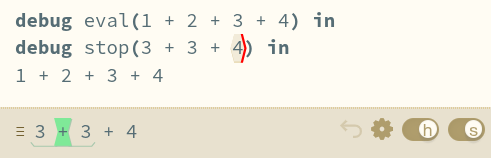
\includegraphics[width=0.4\textwidth]{images/filter-example-user-select.png}}
  \Description{Stepper UI showing the expression 1 + 2 + 3 + 4 with a highlighted subexpression selection and control buttons.}
  \caption{Stepper UI at the user-selection step.}\label{fig:simple_example_final_ui}
\end{figure}

\subsection{Semantics for Contextual Dynamics}\label{sec:dynamics}

We now present the formal rules that define each phase, building
up to the top-level stepping judgment.

\subsubsection{Instrumentation.} The instrumentation judgment traverses
an expression, testing each sub-expression against the current filter's
pattern using the matching judgment \(\Matches{p}{e}\). When a match is found (the ``-Y'' rules), a residue is
inserted; otherwise (the ``-N'' rules), the sub-expression is left
unchanged. When a nested filter is encountered, its priority is
incremented so that inner filters take precedence.

\fbox{\(\InstructPAGL{p}{a}{g}{l}{e}{e'}\)} \(e\) is dynamically instrumented to \(e'\).
\begin{mathpar}
  \inferrule[I-V]{
    \Value{v}
  }{
    \InstructPAGL{p}{a}{g}{l}{v}{v}
  } \qquad
  \inferrule[I-Var]{
  }{
    \InstructPAGL{p}{a}{g}{l}{x}{x}
  } \\
  \inferrule[I-Filter]{
    \InstructF{(p_0, a_0, g_0, l_0)}{e_0}{e} \\
    \InstructF{(p, a, g, l_0 + 1)}{e}{e'}
  }{
    \InstructF{(p_0, a_0, g_0, l_0)}{\Filter{(p, a, g)}{e_0}}{\Filter{(p, a, g)}{e'}}
  } \\
  \inferrule[I-Residue]{
    \InstructF{(p_0, a_0, g_0, l_0)}{e_0}{e} \\
  }{
    \InstructF{(p_0, a_0, g_0, l_0)}{\Residue{a}{g}{l}{e_0}}{\Residue{a}{g}{l}{e}}
  } \\
  \inferrule[I-Fix]{
    \
  }{
    \InstructPAGL{p}{a}{g}{l}{\Fix{x}{e}}{\Fix{x}{e}}
  } \\
  \inferrule[I-Ap-Y]{
    \InstructPAGL{p}{a}{g}{l}{e_1}{e_1'} \\
    \InstructPAGL{p}{a}{g}{l}{e_2}{e_2'} \\
    \Matches{p}{e_1(e_2)}
  }{
    \InstructPAGL{p}{a}{g}{l}{e_1(e_2)}{\Residue{a}{g}{l}{e_1'(e_2')}}
  } \\
  \inferrule[I-Ap-N]{
    \InstructPAGL{p}{a}{g}{l}{e_1}{e_1'} \\
    \InstructPAGL{p}{a}{g}{l}{e_2}{e_2'} \\
    \DoesNotMatch{p}{e_1(e_2)}
  }{
    \InstructPAGL{p}{a}{g}{l}{e_1(e_2)}{e_1'(e_2')}
  } \\
  \inferrule[I-Add-Y]{
    \InstructPAGL{p}{a}{g}{l}{e_1}{e_1'} \\
    \InstructPAGL{p}{a}{g}{l}{e_2}{e_2'} \\
    \Matches{p}{e_1 + e_2}
  }{
    \InstructPAGL{p}{a}{g}{l}{e_1 + e_2}{\Residue{a}{g}{l}{e_1' + e_2'}}
  } \\
  \inferrule[I-Add-N]{
    \InstructPAGL{p}{a}{g}{l}{e_1}{e_1'} \\
    \InstructPAGL{p}{a}{g}{l}{e_2}{e_2'} \\
    \DoesNotMatch{p}{e_1 + e_2}
  }{
    \InstructPAGL{p}{a}{g}{l}{e_1 + e_2}{e_1' + e_2'}
  } \\
\end{mathpar}

Instrumentation is the cost center of a step: each step re-instruments
the entire subtree, and because residues persist across steps, these
re-instruments leave more and more residues in the expression. and the
optimization pass below exists to keep that work from compounding across
steps.

\subsubsection{Pattern matching.} The matching judgment determines
when a sub-expression's structure conforms to a filter's pattern.
Because filter and residue wrappers are purely instrumental, matching
ignores them by comparing expression bodies modulo the stripping
operation defined below.

\fbox{\(\Matches{p}{e}\)} Pattern \(p\) matches expression \(e\).
\begin{mathpar}
  \inferrule[M-All]{\ }{
    \Matches{\$e}{e}
  } \qquad
  \inferrule[M-Val]{\Value{v}}{
    \Matches{\$v}{v}
  } \qquad
  \inferrule[M-Nat]{
    \
  }{
    \Matches{\Nat{n}}{\Nat{n}}
  } \\
  \inferrule[M-Lam]{
    \Strip{e_1} \equiv \Strip{e_2}
  }{
    \Matches{\Lam{x_1}{e_1}}{\Lam{x_2}{e_2}}
  } \qquad
  \inferrule[M-Fix]{
    \Strip{e_1} \equiv \Strip{e_2}
  }{
    \Matches{\Fix{x_1}{e_1}}{\Fix{x_2}{e_2}}
  } \\
  \inferrule[M-Ap]{
    \Matches{p_1}{e_1} \\
    \Matches{p_2}{e_2}
  }{
    \Matches{p_1(p_2)}{e_1(e_2)}
  } \qquad
  \inferrule[M-Add]{
    \Matches{p_1}{e_1} \\
    \Matches{p_2}{e_2}
  }{
    \Matches{p_1 + p_2}{e_1 + e_2}
  }
\end{mathpar}

\subsubsection{Stripping.} The strip operation erases all filter and
residue wrappers from an expression. It is used by \textsc{M-Lam} and
\textsc{M-Fix} to compare expression bodies modulo instrumentation.

\fbox{\(\Strip{e} = {e'}\)} Strip filter and residue wrappers from expression \(e\).
\[
  \begin{aligned}
    \Strip{x} &= x \\
    \Strip{\Lam{x}{e}} &= \Lam{x}{\Strip{e}} \\
    \Strip{(e_1(e_2))} &= (\Strip{e_1})(\Strip{e_2}) \\
    \Strip{\Nat{n}} &= \Nat{n} \\
    \Strip{(e_1 + e_2)} &= (\Strip{e_1}) + (\Strip{e_2}) \\
    \Strip{(\Filter{f}{e})} &= \Strip{e} \\
    \Strip{\Residue{a}{g}{l}{e}} &= \Strip{e} \\
    \Strip{\Fix{x}{e}} &= \Fix{x}{\Strip{e}}
  \end{aligned}
\]

\subsubsection{Decay.} After a step is taken, one-shot residues
(\(\GasOne\)) are removed while persistent residues (\(\GasAll\)) are
preserved for future steps:

\fbox{\(\Decay{\mathcal{E}} = \mathcal{E}'\)} Evaluation context \(\mathcal{E}\) decays to context \(\mathcal{E}'\).
\[
  \begin{aligned}
    \Decay{x} &= x \\
    \Decay{\Lam{x}{e}} &= \Lam{x}{\Decay{e}} \\
    \Decay{e_1(e_2)} &= (\Decay{e_1})(\Decay{e_2}) \\
    \Decay{\Nat{n}} &= \Nat{n} \\
    \Decay{e_1 + e_2} &= (\Decay{e_1}) + (\Decay{e_2}) \\
    \Decay{\Filter{(p, a, g)}{e}} &= \Filter{(p, a, g)}{\Decay{e}} \\
    \Decay{\Residue{a}{\GasOne}{l}{e}} &= \Decay{e} \\
    \Decay{\Residue{a}{\GasAll}{l}{e}} &= \Residue{a}{\GasAll}{l}{\Decay{e}}
  \end{aligned}
\]

\subsubsection{Action selection.} The analysis judgment walks outward
through the evaluation context, comparing residue priorities to
determine whether to step or skip. When a residue has higher priority
than the current action, it takes over; otherwise, the existing action
is kept:

\fbox{\(\Analyze{(a, l)}{\mathcal{E}}{a'}\)} Under action \((a, l)\), context \(\mathcal{E}\) yields action \(a'\).
\begin{mathpar}
  \inferrule[A-Var]{
  }{
    \Analyze{(a, l)}{\circ}{a}
  } \\
  \inferrule[A-Ap-L]{
    \Analyze{(a, l)}{\mathcal{E}_1}{a'}
  }{
    \Analyze{(a, l)}{\mathcal{E}_1(e)}{a'}
  } \qquad
  \inferrule[A-Ap-R]{
    \Analyze{(a, l)}{\mathcal{E}_2}{a'}
  }{
    \Analyze{(a, l)}{e_1(\mathcal{E}_2)}{a'}
  } \\
  \inferrule[A-Add-L]{
    \Analyze{(a, l)}{\mathcal{E}_1}{a'}
  }{
    \Analyze{(a, l)}{\mathcal{E}_1 + e}{a'}
  } \qquad
  \inferrule[A-Add-R]{
    \Analyze{(a, l)}{\mathcal{E}_2}{a'}
  }{
    \Analyze{(a, l)}{e_1 + \mathcal{E}_2}{a'}
  } \\
  \inferrule[A-Filter]{
    \Analyze{(a, l)}{\mathcal{E}}{a'}
  }{
    \Analyze{(a, l)}{\Filter{f}{\mathcal{E}}}{a'}
  } \\
  \inferrule[A-Residue-One-Old]{
    l \le l_0 \\
    \Analyze{(a_0, l_0)}{\mathcal{E}}{a'}
  }{
    \Analyze{(a_0, l_0)}{\Residue{a}{\GasOne}{l}{\mathcal{E}}}{a'}
  } \qquad
  \inferrule[A-Residue-One-New]{
    l > l_0 \\
    \Analyze{(a, l)}{\mathcal{E}}{a'}
  }{
    \Analyze{(a_0, l_0)}{\Residue{a}{\GasOne}{l}{\mathcal{E}}}{a'}
  } \\
  \inferrule[A-Residue-All-Old]{
    l \le l_0 \\
    \Analyze{(a_0, l_0)}{\mathcal{E}}{a'}
  }{
    \Analyze{(a_0, l_0)}{\Residue{a}{\GasAll}{l}{\mathcal{E}}}{a'}
  } \qquad
  \inferrule[A-Residue-All-New]{
    l > l_0 \\
    \Analyze{(a, l)}{\mathcal{E}}{a'}
  }{
    \Analyze{(a_0, l_0)}{\Residue{a}{\GasAll}{l}{\mathcal{E}}}{a'}
  } \\
\end{mathpar}

The remaining judgments---evaluation contexts, values, substitution, decomposition
(\fbox{\(\Decompose{e}{\mathcal{E}}{e'}\)}), composition
(\fbox{\(\Compose{e}{\mathcal{E}}{e'}\)}), and instruction transition
(\fbox{\(\Transition{e}{e'}\)})---are standard extensions of
the lambda calculus with filter and residue frames.
The full rules are given in Appendix~\ref{sec:standard_rules}.

\subsubsection{Optimization.} Instrumentation can stack adjacent
residues around a single redex when several nested filters match it,
and those residues persist into the next step. The optimization pass
collapses adjacent residues to the highest-priority survivor at each
nesting level---the same residue that action selection would have
consulted---so the collapse is observationally invisible. We discuss
the cost of instrumentation and the asymptotic effect of this pass in
Section~\ref{sec:impl-perf}.

\fbox{\(\IsResidue{e}\)} \(e\) is a residue.
\begin{mathpar}
  \inferrule[Is-Residue]{
    \
  }{
    \IsResidue{\Residue{a}{g}{l}{e}}
  }
\end{mathpar}

\fbox{\(\Optimize{e}{e'}\)} \(e\) is optimized to \(e'\)
\begin{mathpar}
  \inferrule[O-Var]{
    \
  }{
    \Optimize{x}{x}
  } \quad
  \inferrule[O-Val]{
    \Value{e}
  }{
    \Optimize{e}{e}
  } \\
  \inferrule[O-Ap]{
    \Optimize{e_l}{e_l'} \\
    \Optimize{e_r}{e_r'}
  }{
    \Optimize{e_l(e_r)}{e_l'(e_r')}
  } \quad
  \inferrule[O-Add]{
    \Optimize{e_l}{e_l'} \\
    \Optimize{e_r}{e_r'}
  }{
    \Optimize{e_l + e_r}{e_l' + e_r'}
  } \\
  \inferrule[O-Filter]{
    \Optimize{e}{e'}
  }{
    \Optimize{\Filter{f}{e}}{\Filter{f}{e'}}
  } \\
  \inferrule[O-Residue-Inner]{
    l_i > l_o \\
    \Optimize{\Residue{a_i}{g_i}{l_i}{e}}{e'}
  }{
    \Optimize{\Residue{a_o}{g_o}{l_o}{\Residue{a_i}{g_i}{l_i}{e}}}{e'}
  } \quad
  \inferrule[O-Residue-Outer]{
    l_i \leq l_o \\
    \Optimize{\Residue{a_o}{g_o}{l_o}{e}}{e'}
  }{
    \Optimize{\Residue{a_o}{g_o}{l_o}{\Residue{a_i}{g_i}{l_i}{e}}}{e'}
  } \quad
  \inferrule[O-Residue-Other]{
    \neg{(\IsResidue{e})} \\
    \Optimize{e}{e'}
  }{
    \Optimize{\Residue{a}{g}{l}{e}}{\Residue{a}{g}{l}{e'}}
  } \\
  \inferrule[O-Fix]{
    \
  }{
    \Optimize{\Fix{x}{e}}{\Fix{x}{e}}
  }
\end{mathpar}

\subsubsection{Stepping judgment.} With all the pieces in place, the
top-level stepping judgment ties the pipeline together.
\textsc{S-Step} fires when action selection yields \(\ActStep\) and
the redex is not a filter/residue elimination (checked by
\(\Strippable{}\)); the step is shown to the user. \textsc{S-Skip}
fires otherwise: the step is performed silently and stepping continues
recursively.

\fbox{\(\Strippable{e}\)} Expression \(e\) is a filter or residue wrapper.
\begin{mathpar}
  \inferrule[F-Filter]{
  }{
    \Strippable{(\Filter{f}{e})}
  } \qquad
  \inferrule[F-Residue]{
  }{
    \Strippable{\Residue{a}{g}{l}{e}}
  }
\end{mathpar}

\fbox{\(\Step{e}{e'}{n}\)} Expression \(e\) steps to \(e'\) in \(n\) steps.
\begin{mathpar}
  \inferrule[S-Step]{
    \InstructPAGL{\PatExpr}{\ActStep}{\GasOne}{0}{e}{e_i} \\
    \Decompose{e_i}{\mathcal{E}_0}{e_0} \\
    \Analyze{(\ActStep, 0)}{\mathcal{E}_0}{\ActStep} \land{} \neg{} (\Strippable{e_0}) \\
    \Transition{e_0}{e_t} \\
    \Compose{e_1}{(\Decay{\mathcal{E}_1})}{e_t}
  }{
    \Step{e}{e_1}{1}
  } \\
  \inferrule[S-Skip]{
    \InstructPAGL{\PatExpr}{\ActStep}{\GasOne}{0}{e}{e_i} \\
    \Decompose{e_i}{\mathcal{E}_0}{e_0} \\
    \Analyze{(\ActStep, 0)}{\mathcal{E}_0}{\ActSkip} \lor \Strippable{e_0}\\
    \Transition{e_0}{e_t} \\
    \Compose{e_1}{(\Decay{\mathcal{E}_1})}{e_t} \\
    \Step{e_1}{e_2}{n}
  }{
    \Step{e}{e_2}{n + 1}
  } \\
  \inferrule[S-Value]{
    \Value{v}
  }{
    \Step{v}{v}{0}
  }
\end{mathpar}

\subsection{Properties}

Because the Filtered Stepper Calculus layers filter and residue annotations on
top of a standard reduction calculus, we want to confirm that these additions
are \emph{conservative}: they should not break the guarantees of the underlying
language. Preservation (Theorem~\ref{thm:preservation}) ensures that every
intermediate state the stepper shows the user has the same type as the original
expression, so the displayed evaluation remains coherent; Progress
(Theorem~\ref{thm:progress}) ensures that the stepper does not introduce new
stuck states for well-typed programs; and Simulation
(Theorem~\ref{thm:simulation}) ensures that the filter machinery only controls
\emph{which} steps are shown, not which reductions are possible, so the
underlying evaluation behavior matches the base Untyped Lambda Calculus.
Preservation and Progress are classically stated over a typed language, so we
state them for a typed variant of the Filtered Stepper Calculus that extends
the syntax with natural number and arrow types; the typing judgment
\(\TypeEntails{\Gamma}{e}{\tau}\) and the rules for expressions and patterns
are standard, with the full static semantics given in
Appendix~\ref{sec:statics}.

\begin{theorem}[Preservation]\label{thm:preservation}
  If an expression has type \(\tau\), then after stepping, the stepped expression also has type \(\tau\).
  \[
    \forall e, \tau, n, \Gamma, \qquad
    \TypeEntails{\Gamma}{e}{\tau} \land \Step{e}{e'}{n} \implies \TypeEntails{\Gamma}{e'}{\tau}
  \]
\end{theorem}

\begin{theorem}[Progress]\label{thm:progress}
  If an expression is well-typed, then there exists an \(n\) such that the expression can be stepped for \(n\) steps.
  \[
    \forall e, \tau, \qquad
    \TypeEntails{\varnothing}{e}{\tau} \implies \exists e' . \Step{e}{e'}{1}
  \]
\end{theorem}

To state the simulation theorem, we define an unfiltered stepping
judgment that ignores all filter and residue annotations:

\fbox{\(\JustStep{e}{e'}{n}\)} Expression \(e\) takes \(n\) steps to \(e'\), ignoring filters and residues.
\begin{mathpar}
  \inferrule[J-Step]{
    \Decompose{e}{\mathcal{E}_0}{e_0} \\
    \Transition{e_0}{e_0'} \\
    \Compose{e'}{\mathcal{E}_0}{e_0'}
  }{
    \JustStep{e}{e'}{1}
  }
\end{mathpar}

\begin{theorem}[Simulation]\label{thm:simulation}
  If an expression \(e\) takes \(n\) steps to become \(e'\), then the stripped-down version of \(e\), which is \(\Strip{e}\), will take \(m\) steps to become \(\Strip{e'}\) for some \(m\).
  \[
    \forall e, n, e', \qquad
    \Step{e}{e'}{n} \implies \exists m, \JustStep{\Strip{e}}{\Strip{e'}}{m}
  \]
\end{theorem}

Preservation and progress hold for a typed variant of the calculus
that extends the syntax with natural number and arrow types. The
typing rules for expressions and patterns are standard; the full
static semantics are given in Appendix~\ref{sec:statics}.

\subsection{Agda Mechanization}

We mechanize both the dynamic and static semantics of the stepper
calculus in Agda, as well as the proofs of the preservation, progress,
and simulation properties stated above. We use de Bruijn indices to
implement \(\alpha\)-equivalence during the filter-matching process.
To mitigate the complexity of de Bruijn indices, we fuse the
operations of substitution and function application into a single
function, eliminating many structurally possible but invalid states
(for example, shifting down a variable with index 0). Additionally,
we use well-founded recursion to prove termination of the
instrumentation and optimization passes.

%%% Local Variables:
%%% mode: LaTeX
%%% TeX-master: "main"
%%% End:
